\documentclass[9pt,letterpaper]{article}
\usepackage{macroshw}
\usepackage{wrapfig}

\begin{document}
\[
	\text{Cylindrical: }\del\psi = \pdiff[\psi]{\rho}\vecth e_1 +\frac{1}{\rho}\pdiff[\psi]{\phi}\vecth e_2+\pdiff[\psi]{z}\vecth e_3,
	\quad \del\cdot \vect A = \frac{1}{\rho}\pdiff{\rho}(\rho A_1)+\frac{1}{\rho}\pdiff[A_2]{\phi}+\pdiff[A_3]{z}
\]
\[
	\del\times\vect A = \plr{\frac{1}{\rho}\pdiff[A_3]{\phi}-\pdiff[A_2]{z}}\vecth e_1+
	\plr{\pdiff[A_1]{z}-\pdiff[A_3]{\rho}}\vecth e_2+\frac{1}{\rho}\plr{\pdiff{\rho}(\rho A_2)-\pdiff[A_1]{\phi}}\vecth e_3
\]
\[
	\del^2\psi = \frac{1}{\rho}\pdiff{\rho}\plr{\rho\pdiff[\psi]{\rho}}+\frac{1}{\rho^2}\pdifff{\psi}{*2\phi}+\pdifff{\psi}{*2z}
\]
\[
	\text{Spherical: }\pdiff[\psi]{r}\vecth e_1 +\frac{1}{r}\pdiff[\psi]{\theta}\vecth e_2+\frac{1}{r\sin\theta}\pdiff[\psi]{\phi}\vecth e_3,
	\quad
	\del\cdot \vect A = \frac{1}{r^2}\pdiff{r}(r^2A_1)+\frac{1}{r\sin\theta}\pdiff{\theta}(\sin\theta A_2)+\frac{1}{r\sin\theta}
	\pdiff[A_3]{\phi}
\]
\[
	\del\times \vect A = \frac{1}{r\sin\theta}\blr{\pdiff{\theta}(\sin\theta A_3)-\pdiff[A_2]{\phi}}\vecth e_1
	+\blr{\frac{1}{r\sin\theta}\pdiff[A_1]{\phi}-\frac{1}{r}\pdiff{r}(rA_3)}\vecth e_2+
	\frac{1}{r}\blr{\pdiff{r}(rA_2)-\pdiff[A_1]{\theta}}\vecth e_3
\]
\[
	\del^2\psi = \frac{1}{r^2}\pdiff{r}\plr{r^2\pdiff[\psi]{r}}+\frac{1}{r^2\sin\theta}\pdiff{\theta}\plr{\sin\theta\pdiff[\psi]{\theta}}+
	\frac{1}{r^2\sin^2\theta}\pdifff{\psi}{*2\phi}
\]
\\
\[
	\vect P\cdot\vecth n  = \sigma_b,
	\quad
	-\del\cdot\vect P = \rho_b,
	\quad
	\epsilon_0\del\cdot\vect E = \rho_b+\rho_f = -\del\cdot\vect P +\rho_f,
	\quad
	\del\cdot(\epsilon_0\vect E+\vect P) = \rho_f
\]
\[
	\del\cdot\vect D = \rho_f,
	\quad 
	\oint \vect D\cdot d\vect S = q_{free},
	\quad
	\vect P = \epsilon_0(\epsilon_r-1)\vect E,
	\quad
	\epsilon = \epo\epsilon_r,
	\quad
	\vect D = \epsilon \vect E
\]
\[
	(\vect D_2-\vect D_1)\cdot \vecth n_{21} = \sigma_f,
	\quad
	(\vect D_2-\vect D_1)\times \vecth n_{21} = (\vect P_2-\vect P_1)\times\vecth n_{21},
\]
\[
	(\vect E_2-\vect E_1)\cdot \vecth n_{21} = \frac{\sigma}{\epo},
	\quad
	(\vect E_2-\vect E_1)\times \vecth n_{21} = 0,
	\quad
	\epsilon_1\vect E_{1n} = \epsilon_2\vect E_{2n}
\]
\begin{align*}W_{int} &= k\sum_{i=1}^n\sum_{j<i}{\frac{q_iq_j}{|\vect x_i-\vect x_j|}}=\frac k2\sum_i^n\sum_{\substack{j\\j\neq i}}\frac{q_iq_j}{|\vect x_i-\vect x_j|}=\frac{1}{2}\sum_{i=1}^nq_i\sum_{\substack{j\\j\neq i}}k\frac{q_j}{|\vect x_i-\vect x_j|}\\
&=\frac 12\sum_{i=1}^nq_i\Phi(\vect x_i)=\frac 12\int_\rho{\rho(\vect x)\Phi(\vect x)\,d^3x}=\frac \epo2\int_{all}{|\vect E|^2\,d^3x}=-\int_\infty^r{\vect F\cdot d\vect l}=\frac 12 q\Phi_*(\vect x)
\end{align*}
\[
	W_{int} = \frac{1}{2}\int \vect B^2\ d^3r,\quad = \frac{1}{2}\int \vect D\cdot\vect E\ d^3r
	\quad
	W_{int\text -dip} = \vect p\cdot\vect E;\quad W_{12} = 
	\frac{\vect p_1\cdot\vect p_2-3(\vect n\cdot \vect p_1)(\vect n\cdot\vect p_2)}{4\pi\epo|\vect x_1-\vect x_2|^3}
\]
\[
	\vect B = \frac{\mu_0}{4\pi}\int \frac{Id\vect l\times(\vect r-\vect r')}{|\vect r-\vect r'|^3},\quad
	\del\times \vect B = \mu_0\vect J,\quad
	\del\cdot\vect B = 0,\quad
	d\vect F = Id\vect l\times\vect B,\quad
	w_B = \frac{B^2}{2\mu_0}
\]
\[
	\vect B = \del\times\vect A,\quad
	\del^2 \vect A = -\mu_0\vect J,\quad
	\vect A(\vect x) = \frac{\mu_0}{4\pi}\int \frac{\vect J(\vect x')}{|\vect x-\vect x'|}d^3x'+C
\]
\[
	B = \frac{\mu_0 I}{4\pi r}(\sin\theta_2-\sin\theta_1)
\]
\begin{wrapfigure}{r}{0.5\textwidth}
    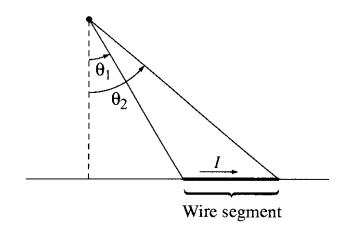
\includegraphics[width=0.48\textwidth]{wire.png}
\end{wrapfigure}
\[
	q' = -\plr{\frac{\epsilon_2-\epsilon_1}{\epsilon_2+\epsilon_1}}q,\quad 
	q'' = \plr{\frac{2\epsilon_2}{\epsilon_2+\epsilon_1}}q
\]
	
	
	
	
	
	
	
\end{document}

